\documentclass[conference]{IEEEtran}
%\documentclass{acm_proc_article-sp}

\makeatletter
\newif\if@restonecol

\let\algorithm\relax
\let\endalgorithm\relax
\usepackage[tight,footnotesize]{subfigure}
\usepackage {paralist}
\usepackage{comment}
\usepackage{array}
\usepackage{amsmath}
\usepackage{graphicx}
\usepackage{amssymb}
\usepackage{cite}
\usepackage{url}
\makeatother
\makeatletter
\providecommand{\tabularnewline}{\\}


\newtheorem{clm}{Claim}
\begin{document}

\title{Length-based Contention Management: Increasing Schedulability of Real-Time Software with STM Concurrency Control}


%\author{Mohammed Elshambakey
%\affil{ECE Dept., Virginia Tech, Blacksburg, VA 24060, USA}
%Binoy Ravindran
%\affil{ECE Dept., Virginia Tech, Blacksburg, VA 24060, USA}
%}

\begin{comment}
\author{\IEEEauthorblockN{Mohammed Elshambakey}
\IEEEauthorblockA{ECE Dept, Virginia Tech\\
Blacksburg, VA 24061, USA\\
Email: shambake@vt.edu}
\and
\IEEEauthorblockN{Binoy Ravindran}
\IEEEauthorblockA{ECE Dept, Virginia Tech\\
Blacksburg, VA 24061, USA\\
Email: binoy@vt.edu}
}
\end{comment}


\maketitle

\begin{abstract}
We consider software transactional memory (STM) concurrency control for multicore real-time software, and present a novel contention manager (CM) for resolving transactional conflicts, called length-based CM (or LCM). We upper bound transactional retries and response times under LCM, when used with G-EDF and  G-RMA schedulers. We identify the conditions under which LCM is superior to previous real-time CMs including those based on dynamic and fixed priorities. %We show that, LCM achieves higher schedulability for larger  atomic section lengths than that with past CMs.
Presented work is analytical as the questions we try to answer is analytical, so our results. Experimental evaluation will be done in future work.
\end{abstract}

%\maketitle

\section{Introduction}
\label{sec:intro}

Lock-based concurrency control suffers from programmability, scalability, and composability challenges~\cite{Herlihy:2006:AMP:1146381.1146382}. These challenges are exacerbated in emerging multicore architectures, on which improved software performance must be achieved by exposing greater concurrency.  Transactional memory (TM) is an alternative synchronization model for shared memory data objects that promises to alleviate these difficulties.  With TM, programmers organize code that read/write shared objects as transactions, which appear to execute atomically. Two transactions conflict if they access the same object and one access is a write. When that happens, a contention manager (or CM)
%~\cite{Guerraoui:2005:TTT:1073814.1073863} 
resolves the conflict by aborting one and allowing the other to proceed to commit, yielding (the illusion of) atomicity. Aborted transactions are re-started.
%often immediately.  
In addition to a simple programming model, TM provides performance comparable to highly concurrent fine-grained locking and lock-free approaches,  
%~\cite{Saha:2006:MHP:1122971.1123001}, 
and is composable. 
%~\cite{Harris:2005:CMT:1065944.1065952}. 
TM has been proposed in hardware, called HTM,  
%(e.g.,~\cite{austenmc:tcc:dissertation:2009}), 
and in software, called STM,  
%(e.g.,~\cite{sha95}),  
with the usual tradeoffs: HTM has lesser overhead, but needs transactional support in hardware; STM is available on any hardware. See~\cite{tm-book10} for an excellent overview on TM.


Given STM's programmability, scalability, and composability advantages, we consider it for concurrency control in multicore real-time software. Doing so requires bounding transactional  retries, as real-time threads, which subsume transactions, must satisfy time constraints.  Retry bounds in STM are dependent on the CM policy at hand (analogous to the way thread response time bounds are scheduler-dependent). 
Thus, real-time CM is logical.

Past research on real-time CM have proposed resolving transactional contention using dynamic and fixed priorities of parent threads, resulting in Earliest-Deadline-First-based CM (ECM) and Rate Monotonic Assignment-based CM (RCM), respectively~\cite{fahmy2009bounding,fahmy2009response,stmconcurrencycontrol:emsoft11}.
These works show that, ECM and RCM, when used with Global EDF (G-EDF) and Global RMA  (G-RMA) schedulers, respectively, achieve higher schedulability than locking and lock-free synchronization techniques only under some ranges for the maximum atomic section length. This raises a fundamental question: is it possible to increase the atomic section length by an alternative CM design, so that STM's schedulability advantage has a larger coverage? 

We answer this question by designing a novel CM that can be used with both dynamic and fixed priority (global) multicore real-time schedulers: length-based CM or LCM (Section~\ref{sec 9.1}). LCM resolves conflicts based on the priority of conflicting jobs, besides the length of the interfering atomic section, and the normalized length of the interfered atomic section.  We establish LCM's retry and response time upper bounds, when used with G-EDF (Section~\ref{response g-edf/lcm}) and with G-RMA (Section~\ref{rma}) schedulers. We identify the conditions under which G-EDF/LCM outperforms ECM (Section~\ref{performance g-edf-lcm}) and G-RMA/LCM outperforms RCM (Section~\ref{rma eval}). 

\begin{comment}
We show that, LCM achieves higher schedulability under larger transaction length 
than that under ECM, 
and increases the minimum upper limit on the ratio between transaction length and retry-loop length from that under RCM. 
This greater schedulability advantage of STM thus allows programmers to reap STM's significant programmability and composability benefits for a broader range of multicore real-time software than what was previously possible.
\end{comment}
\section{Related Work}
\label{sec:past}

Transactional-like concurrency control without using locks, for real-time systems, has been previously studied in the context of non-blocking data structures (e.g.,~\cite{anderson95realtime}). Despite their numerous advantages over locks 
(e.g., deadlock-freedom), 
their programmability has remained a challenge. 
Past studies show that they are best suited for simple data structures where their retry cost is competitive to the cost of lock-based synchronization~\cite{bc+08}.  In contrast, STM is semantically simpler~\cite{Herlihy:2006:AMP:1146381.1146382}, and is often the only viable lock-free solution for complex data structures (e.g., red/black tree)~\cite{key-1} and nested critical sections~\cite{Saha:2006:MHP:1122971.1123001}.

STM concurrency control for real-time systems has been previously studied in~\cite{manson2006preemptible,fahmy2009bounding,sarni2009real,schoeberl2010rttm,key-1,barrosmanaging,stmconcurrencycontrol:emsoft11}.


\cite{manson2006preemptible} proposes a restricted version of STM for uniprocessors. Uniprocessors do not need contention management.

\cite{fahmy2009bounding} bounds response times in distributed multiprocessor systems with STM synchronization. They consider Pfair scheduling, limit to small atomic regions with fixed size, and limit transaction execution to span at most two quanta. In contrast, we allow transaction lengths 
with  arbitrary duration. 

\cite{sarni2009real} presents real-time scheduling of transactions and serializes transactions based on deadlines. However, the work does not bound retries and response times. In contrast, we establish such bounds.


\cite{schoeberl2010rttm} proposes real-time HTM. The work does not describe how transactional conflicts are resolved. Besides, the retry bound assumes that the worst case conflict between atomic sections of different tasks occurs when the sections are released at the same time. However, we show that this is not the worst case. We develop retry and response time upper bounds based on much worse conditions.


\cite{key-1} upper bounds retries and response times for  ECM with G-EDF, and identify the tradeoffs against locking and lock-free protocols. Similar to~\cite{schoeberl2010rttm},~\cite{key-1} also assumes that the worst case conflict between atomic sections occurs when the sections are released simultaneously. 

The ideas in~\cite{key-1} are extended in~\cite{barrosmanaging}, which presents three real time CM designs. But no retry bounds nor schedulability analysis techniques are presented for those CMs. 

\cite{stmconcurrencycontrol:emsoft11} presents the ECM and RCM contention managers, and upper bounds transactional retries and response times under them. The work also identifies the conditions under which ECM and RCM are superior to locking and lock-free techniques. In particular, they show that, the STM superiority holds only under some ranges for the maximum atomic section length. Our work builds upon this result.

\section{Preliminaries}
\label{sec:model}

We consider a multiprocessor system with $m$ identical processors and $n$ sporadic tasks $\tau_1, \tau_2,\ldots, \tau_n$. The $k^{th}$ instance (or job) of a task $\tau_i$ is denoted $\tau_i^k$. Each task $\tau_i$ is specified by its worst case execution time (WCET) $c_i$, its minimum period $T_i$ between any two consecutive instances, and its relative deadline $D_i$, where $D_i=T_i$. Job $\tau_i^j$ is released at time $r_i^j$ and must finish no later than its absolute deadline $d_i^j=r_i^j+D_i$. Under a fixed priority scheduler such as G-RMA, $p_i$ determines $\tau_i$'s (fixed) priority and it is constant for all instances of $\tau_i$. Under a dynamic priority scheduler such as G-EDF, a $\tau_i^j$'s priority, $p_i^j$, is determined by its absolute deadline. 
A task $\tau_j$ may interfere with task $\tau_i$ for a number of times during an interval $L$, and this number is denoted as $G_{ij}(L)$. 
$\tau_j$'s workload that interferes with $\tau_i$ during $L$ is denoted $W_{ij}(L)$.


\textit{Shared objects.} A task may need to access (i.e., read, write) shared, in-memory objects while it is executing any of its atomic sections, which are synchronized using STM. 
The set of atomic sections of task $\tau_i$ is denoted $s_i$. $s_i^k$ is the $k^{th}$ atomic section of $\tau_i$. 
Each object, $\theta$, can be accessed by multiple tasks. The set of objects accessed by $\tau_i$ is $\theta_i$ without repeating objects.
The set of atomic sections used by $\tau_i$ to access $\theta$ is $s_i(\theta)$, and the sum of the lengths of those atomic sections is $len(s_i(\theta))$. $s_i^k(\theta)$ is the $k^{th}$ atomic section of $\tau_i$ that accesses $\theta$. $s_i^k(\theta)$  executes for a duration $len(s_i^k(\theta))$.
% which is the whole length of the atomic section (and not just the part that accesses $\theta$). 
%Thus, for two objects $\theta_1$ and $\theta_2$ that are accessed within the same atomic section of $T_i$, $len(s_i^k(\theta1))=len(s_i^k(\theta2))$. 
If $\theta$ is shared by multiple tasks, then $s(\theta)$ is the set of atomic sections of all tasks accessing $\theta$, and the set of tasks sharing $\theta$ with $\tau_i$ is denoted $\gamma_i(\theta)$. Atomic sections are non-nested, and each atomic section is assumed to access only one object to be consistent with the assumptions made in~\cite{stmconcurrencycontrol:emsoft11} that enabled comparison with retry-loop lock-free approach \cite{key-5}.

The maximum-length atomic section in $\tau_i$ that accesses $\theta$ is denoted $s_{i_{max}} (\theta)$, while the maximum one among all tasks is $s_{max} (\theta)$, and the maximum one among tasks with priorities lower than that of $\tau_i$ is $s_{max}^i (\theta)$.

\textit{STM retry cost.} If two or more atomic sections conflict, the CM will commit one section and abort and retry the others, increasing the time to execute the aborted sections. The increased time that an atomic section $s_i^p (\theta)$ will take to execute due to conflict with another section $s_j^k (\theta)$, is denoted $W_{i}^{p}(s_{j}^{k}(\theta))$. If an atomic section, $s_i^p$, is already executing, and another atomic section $s_j^k$ tries to access a shared object with $s_i^p$, then $s_j^k$ is said to "interfere" or "conflict" with $s_i^p$, and $s_j^k$ is the "interfering job", while $s_i^p$ is the "interfered job".

The total time that a task $\tau_i$'s atomic sections have to retry is denoted $RC(\tau_i)$.
When this retry cost is calculated over the task period $T_i$ or an interval $L$, it is   denoted, respectively, as $RC(T_i)$ and $RC_i(L)$. 

\section{Length-based Contention Manager (LCM)}

LCM resolves conflicts based on the priority of conflicting jobs, besides the length of the interfering atomic section, and the normalized length of the interfered atomic section. So, its design is less straight forward than ECM and RCM~\cite{stmconcurrencycontrol:emsoft11} as they depend only on the priority of the conflicting jobs. This modification in design allows lower priority jobs, under LCM, to retry for less time than ECM and RCM, but higher priority jobs, sometimes, wait for lower priority ones, but this will not result in priority inversion as will be illustrated.

\subsection{\label{sec 9.1} LCM: Design and Rationale}

For both ECM and RCM, $s_{i}^{k}(\theta)$ can be totally repeated if $s_{j}^{l}(\theta)$ --- which belongs to a higher priority job $\tau_{j}^b$ than $\tau_{i}^a$ --- conflicts with $s_{i}^{k}(\theta)$
at the end of its execution, while $s_{i}^{k}(\theta)$ is just about
to commit. Thus, LCM  uses the remaining length of $s_{i}^{k}(\theta)$ when it is interfered,
as well as $len(s_{j}^{l}(\theta))$, to decide which transaction must be aborted. If $s_i^k (\theta)$ is the one which interferes with $s_j^l (\theta)$, then $s_j^l (\theta)$ commits because it belongs to the higher priority job and it because it started before $s_i^k (\theta)$.

We assume that 
\begin{equation}
len(s_{j}^{l}(\theta))=c_{m}len(s_{i}^{k}(\theta))
\label{cm_eq}\end{equation}
where $c_{m}\in]0,\infty[$, to cover all possible lengths of $s_{j}^{l}(\theta)$.
Our idea is to reduce the opportunity for the abortion of $s_{i}^{k}(\theta)$ if it is close to committing when interfered, and $len(s_{j}^{l}(\theta))$ is large. This abortion opportunity is reduced more and more as $s_{i}^{k}(\theta)$ gets closer to its end of execution, or $len(s_{j}^{l}(\theta))$ gets larger. 

On the other side, as $s_{i}^{k}(\theta)$ is interfered early,
or $len(s_{j}^{l}(\theta))$ is small compared to $s_{i}^{k}(\theta)$'s remaining length, the abortion opportunity 
is increased even if $s_i^k (\theta)$ is close to its end of execution. To decide whether $s_{i}^{k}(\theta)$ should be 
aborted or not, we use a threshold value $\psi\in[0,1]$, that determines
the length percentage of $s_{i}^{k}(\theta)$ below which $s_{i}^{k}(\theta)$ will abort due to $s_{j}^{l}(\theta)$.
%
This percentage value is denoted $\alpha^{jl}$ as it differs according to $s_j^l$. 
%
If the abort percent is 0, it means not to abort, and 1 means to abort. 


%
\begin{figure}[htbp]
\centering
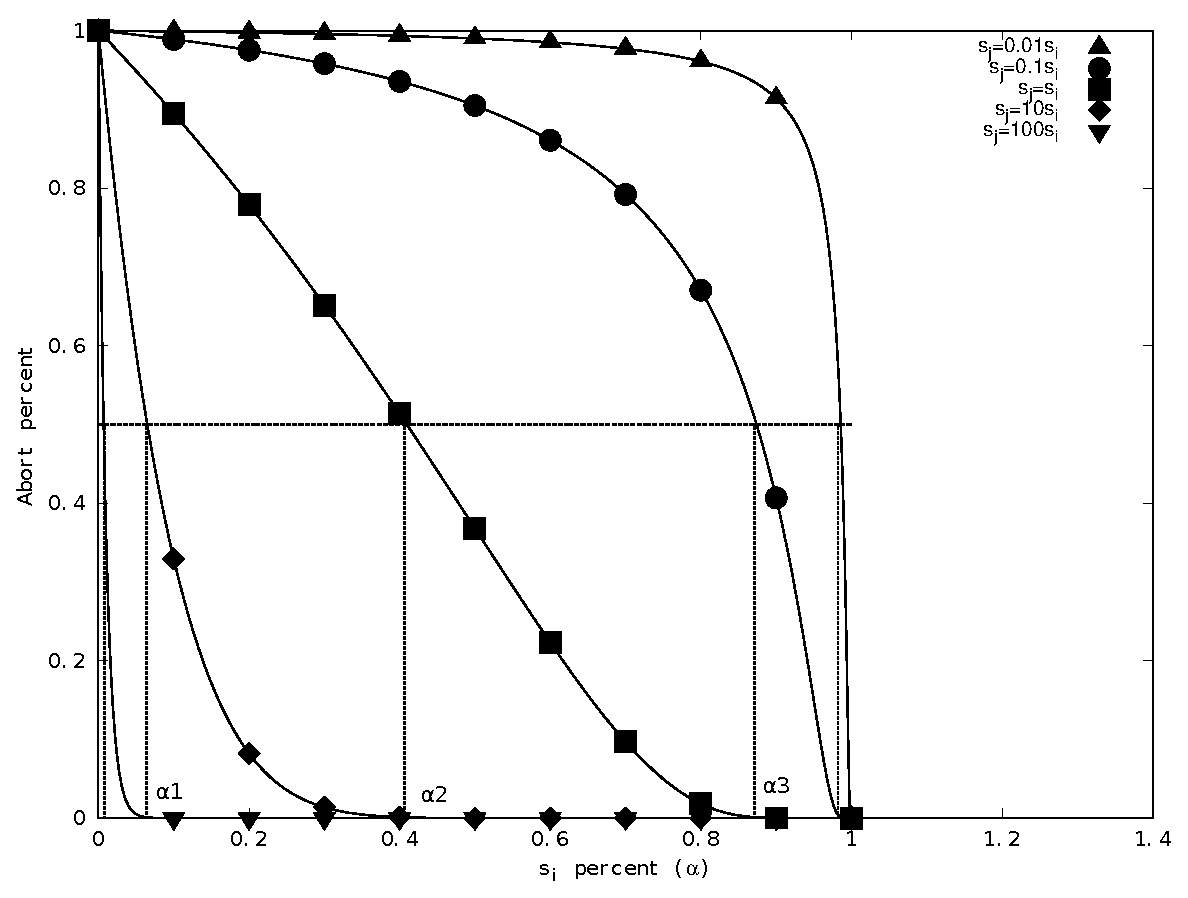
\includegraphics[scale=0.4]{figures/figure16}
\caption{\label{fig16}Interference of $s_{i}^{k}(\theta)$ by various lengths of 
$s_{j}^{l}(\theta)$}
\end{figure}

The behavior of LCM  is illustrated in Figure \ref{fig16}. The figure represents five different lengths of $s_{j}^{l}(\theta)$
interfering with $s_{i}^{k}(\theta)$ at all points of $s_{i}^{k}(\theta)$.
For a specific curve (which means a specific length for $s_{j}^{l}(\theta)$),
$\psi$ determines the percentage of $len(s_{i}^{k}(\theta))$
below which $s_{i}^{k}(\theta)$ will be aborted. For example, for
$len(s_{j}^{l}(\theta))=0.1\times len(s_{i}^{k}(\theta))$, $s_{i}^{k}(\theta)$
will be aborted by $s_{j}^{l}(\theta)$ if the latter interferes with
$s_{i}^{k}(\theta)$ no later than $s_{i}^{k}(\theta)$ reaches $\alpha3$
percentage of its length ($\alpha3$ is shown in Figure~\ref{fig16}). After that, $s_{j}^{l}(\theta)$ will have
to retry. As $len(s_{j}^{k}(\theta))$ decreases, the opportunity
that it will abort $s_{i}^{k}(\theta)$ at a higher percentage $\alpha_{max}$
increases (as illustrated in Figure~\ref{fig16}, $\alpha3>\alpha2>\alpha1$ for reduced length of $s_j^l(\theta)$). The function that is used to represent the 
different curves in Figure \ref{fig16} is:
 \begin{equation}
f(c_{m},\alpha)=e^{\frac{-c_{m}\alpha}{1-\alpha}}\label{eq49}\end{equation}
where $c_{m}$ is fixed for a specific curve and is calculated by~(\ref{cm_eq}), but $\alpha$ changes
along each curve, with a specific value of $\alpha$ corresponds to $\psi$. This function achieves the desired requirement 
that the abortion opportunity is reduced as $s_{i}^{k}(\theta)$ gets
closer to its end of execution (as $\alpha\rightarrow1,\, f(c_{m},1)\rightarrow0$),
or as the length of the conflicting transaction is large (as $c_{m}\rightarrow\infty,\, f(\infty,\alpha)\rightarrow0$).
Meanwhile, this abortion opportunity is increased as $s_{i}^{k}(\theta)$
is interfered closer to its release (as $\alpha\rightarrow0,\, f(c_{m},0)\rightarrow1$),
or as the length of the conflicting transaction decreases (as $c_{m}\rightarrow0,\, f(0,\alpha)\rightarrow1$).
Note that all lengths of $s_{i}^{k}(\theta)$ are normalized
to the same unit length. This way, different values of $s_{j}^{l}(\theta)$
interfere with 
different lengths of $s_{i}^{k}(\theta)$ at the same percentage
$\alpha^{jl}$, but the actual length of the interference 
for different
lengths of $s_{i}^{k}(\theta)$ differ according to $len(s_{i}^{k}(\theta))$ i.e., let $len(s_{i}^{k}(\theta))\ne len(s_{i}^{k+1}(\theta))$. Then, for one $s_{j}^{l}(\theta)$, both $s_{i}^{k}(\theta)$ and $s_{i}^{k+1}(\theta)$
will be interfered at the same value $\alpha^{jl}$, but $\alpha^{jl}len(s_{i}^{k}(\theta))$
differs from $\alpha^{jl}len(s_{i}^{k+1}(\theta))$. The normalization
of different lengths of $s_{i}^{k}(\theta)$ is done to simplify calculations.

As $s_{j}^{l}(\theta)$ belongs to a higher priority job than $s_{i}^{k}(\theta)$, if $s_{j}^{l}(\theta)$ starts before or at the same start time of
$s_{i}^{k}(\theta)$, then $s_{i}^{k}(\theta)$ will have to abort
and retry until $s_{j}^{l}(\theta)$ finishes execution. But if $s_{j}^{l}(\theta)$
starts after $s_{i}^{k}(\theta)$, then the comparison illustrated
previously will be applied. LCM, ECM and RCM are not central CMs, which means each two transactions have to decide which one of them is to commit.

\begin{clm}
\label{LCM_higher_rc}
Let $s_{j}^{l}(\theta)$ interfere with $s_{i}^{k}(\theta)$ at $\alpha^{jl}$
percentage which corresponds to the threshold value $\psi$. Then, the maximum contribution of $s_{j}^{l}(\theta)$ to the retry cost of $s_{i}^{k}(\theta)$ is:
\begin{equation}
W_i^k(s_j^l(\theta))\le \alpha^{jl}len\Big(s_{i}^{k}(\theta)\Big)+len\Big(s_{j}^{l}(\theta)\Big)\label{eq47}\end{equation}
\end{clm}
\begin{proof}
If $s_{j}^{l}(\theta)$ interferes with $s_{i}^{k}(\theta)$
at a $\Upsilon$ percentage, where $\Upsilon<\alpha^{jl}$,
then the retry cost of $s_{i}^{k}(\theta)$ will be $\Upsilon len(s_{i}^{k}(\theta))+len(s_{j}^{l}(\theta))$, which is lower than that calculated in (\ref{eq47}). Besides, 
if $s_{j}^{l}(\theta)$ interferes with $s_{i}^{k}(\theta)$ after
$\alpha^{jl}$ percentage, then $s_{i}^{k}(\theta)$ will not
abort.
\end{proof}

\begin{clm}
\label{LCM_lower_rc}
An atomic section of a higher priority job, $\tau_{j}^b$, may have to abort and retry due to a lower priority job	, $\tau_{i}^a$, if $s_{j}^{l}(\theta)$ interferes
with $s_{i}^{k}(\theta)$ after the $\alpha^{jl}$ percentage.
This retrial time of $\tau_{j}$, due to $s_{i}^{k}(\theta)$ and $s_{j}^{l}(\theta)$,
is upper bounded by:
 \begin{equation}
W_j^l(s_i^k(\theta))\le \Big(1-\alpha^{jl}\Big)len\Big(s_{i}^{k}(\theta)\Big)\label{eq48}\end{equation}
\end{clm}
\begin{proof}
It is derived directly from Claim~\ref{LCM_higher_rc}, as $s_j^l(\theta)$ will have to retry for the remaining length of $s_i^k(\theta)$.
\end{proof}

\begin{clm}
\label{priority_inversion}
A higher priority job, $\tau_i^k$, suffers from priority inversion for at most number of atomic sections in $\tau_i^k$.
\end{clm}
\begin{proof}
Assuming three atomic sections, $s_i^k(\theta)$, $s_j^l(\theta)$ and $s_a^b(\theta)$, where $p_j > p_i$ and $s_j^l(\theta)$ interferes with $s_i^k(\theta)$ after $\alpha^{jl}$ that corresponds to $\psi$. Then $s_j^l(\theta)$ will have to abort and retry. At this time, if $s_a^b(\theta)$ interferes with the other two atomic sections, and the LCM decides which transaction to commit based on comparison between each two transactions. So, we have the following cases:-
\begin{itemize}
\item $p_a < p_i < p_j$, then $s_a^b(\theta)$ will not abort any one because it is still in its beginning and it is of the lowest priority. So. $\tau_j$ is not indirectly blocked by $\tau_a$.
\item $p_i<p_a<p_j$ and even if $s_a^b(\theta)$ interferes with $s_i^k(\theta)$ before $\alpha^{ab}$ that corresponds to the threshold value $\psi$. So, $s_a^b(\theta)$ is allowed abort $s_i^k(\theta)$. But comparison between $s_j^l(\theta)$ and $s_a^b(\theta)$ will result in LCM choosing $s_j^l(\theta)$ to commit and abort $s_a^b(\theta)$ because the latter is still beginning, and $\tau_j$ is of higher priority. If $s_a^b(\theta)$ is not allowed to abort $s_i^k(\theta)$, the situation is still the same, because $s_j^l(\theta)$ was already retrying until $s_i^k(\theta)$ finishes, and when it is time to compare between $s_j^l(\theta)$ and $s_a^b(\theta)$, $s_j^l(\theta)$ will be chosen because it is of higher priority.
\item $p_a>p_j>p_i$, then if $s_a^b(\theta)$ is chosen to commit, this is not priority inversion for $\tau_j$ because $\tau_a$ is of higher priority.
\item if $\tau_a$ preempts $\tau_i$, then LCM will compare only between $s_j^l(\theta)$ and $s_a^b(\theta)$. If $p_a<p_j$, then $s_j^l(\theta)$ will commit because of its task's higher priority and $s_a^b(\theta)$ is still at its beginning, otherwise, $s_j^l(\theta)$ will retry, but this will not be priority inversion because $\tau_a$ is already of higher priority than $\tau_j$.
\end{itemize}
So, by generalizing these cases to any number of conflicting jobs, it is seen that when an atomic section, $s_j^l(\theta)$, of a higher priority job is in conflict with a number of atomic sections belonging to lower priority jobs, $s_j^l(\theta)$ can suffer from priority inversion by only one of them, so if each atomic section belonging to the higher priority job suffers from priority inversion, Claim follows.
\end{proof}

\subsection{\label{response g-edf/lcm} Response time of G-EDF/LCM}

It is desired to determine the response time when LCM is used with G-EDF. So, the following claims are introduced.

\begin{clm}\label{GEDF/LCM response time}
When all instances of $\tau_h$ interfering with one instance of $\tau_i$, $\tau_i^x$, are of higher priority than $\tau_i^x$ (as shown in Figure~\ref{fig17-a}), then the retry cost of $\tau_i$ over $T_i$ due to these instances of $\tau_h$ is upper bounded by
\begin{eqnarray}
\Phi_i(h) & = & \sum_{\theta \in \theta_i \wedge \theta_h}\Bigg(\left\lceil\frac{T_{i}}{T_{h}}\right\rceil\sum_{\forall s_{h}^{l}(\theta)}len\Big(s_{h}^{l}(\theta)\Big)\nonumber\\
& + & \alpha_{max}^{hl}len\Big(s_{max}^{*}(\theta)\Big)\Bigg)
\label{eq78}\end{eqnarray} 

where $s_{max}^* (\theta)$ is the maximum length atomic section, not associated with $\tau_h$, that accesses $\theta$. And  $\alpha_{max}^{hl}$ is $\alpha$ value that corresponds to $\psi$ due to interference of $s_{max}^*(\theta)$ by $s_h^l(\theta)$.
\end{clm}

\begin{proof}
If the absolute deadline of one instance of $\tau_h$, $\tau_h^p$ as shown in Figure~\ref{fig17-a}, coincides with the absolute deadline of $\tau_i^x$, then all interfering instances of $\tau_h$ with $\tau_i^x$ will have a higher priority than $\tau_i^x$, and Claim~\ref{LCM_higher_rc} will be used to determine the retry cost of each atomic section in $\tau_i^x$ due to atomic sections in $\tau_h$. By combining Claim 2 in~\cite{stmconcurrencycontrol:emsoft11} (noting that~(\ref{eq78}) is an upper bound for both $\Phi_1$ and $\Phi_2$ in Claim 2 in~\cite{stmconcurrencycontrol:emsoft11}), then Claim follows.
\end{proof}

\begin{clm}\label{max block}
For an instance $\tau_i^x$ interfered by multiple instances of $\tau_h$, and the last interfering instance, $\tau_h^p$, has a larger absolute deadline than $\tau_i^x$ as shown in Figure~\ref{fig17-b}. Then the retry cost of $\tau_i$ due to interfering instances of $\tau_h$ over $T_i$ is calculated as
\begin{eqnarray}
\Phi_i^*(h) & = & \sum_{\theta \in \theta_i \wedge \theta_h}\Bigg(\left\lfloor\frac{T_{i}}{T_{h}}\right\rfloor\sum_{\forall s_{h}^{l}(\theta)}len\Big(s_{h}^{l}(\theta)\Big)\nonumber\\
& + & \alpha_{max}^{hl}len\Big(s_{max}^{*}(\theta)\Big)\Bigg)\nonumber\\
& + & \sum_{\forall s_{i}^{y}(\theta)}\Big(1-\alpha^{iy}\Big)len\Big(s_{h_{max}}(\theta)\Big)  
\label{eq53}\end{eqnarray} 
where the first and second sums are the same as that calculated by~(\ref{eq78}) except it only includes the contribution of instance $\tau_h^1$ to $\tau_h^{p-1}$ instead of instances $\tau_h^1$ to $\tau_h^p$, the third sum is the upper bound on retry cost of $\tau_i^x$ due to atomic section in $\tau_h^p$, and $\alpha^{iy}$ is the $\alpha$ value that corresponds to $\psi$ for atomic section $s_i^y(\theta)$.
\end{clm}
%
\begin{proof}
Under G-EDF, there can only be at most one instance of $\tau_{h}$, $\tau_{h}^{p}$, interfering with $\tau_i^x$, that can have a lower priority (i.e., larger absolute deadline) than $\tau_{i}^{x}$. This is obtained by shifting Figure~\ref{fig17-a} to the right to give Figure~\ref{fig17-b}. While $\tau_h^p$ cannot affect the non-atomic operation of $\tau_i^x$, because of its lower priority, $\tau_h^p$ can abort and retry atomic sections of $\tau_i^x$.

%
\begin{figure}
\subfigure[\label{fig17-a}$\tau_h^p$ has a higher priority than $\tau_i^x$]{
\begin{centering}
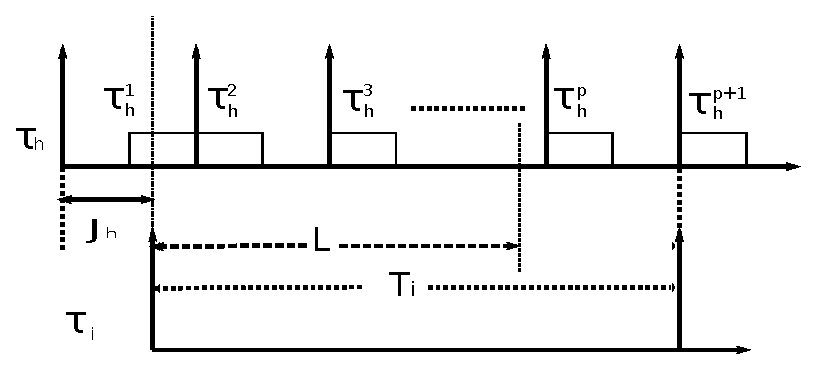
\includegraphics[scale=0.5]{figures/figure17-a}
\par\end{centering}
}
\subfigure[\label{fig17-b}$\tau_{h}^{p}$ has lower priority than $\tau_i^x$]{
\begin{centering}
\includegraphics[scale=0.5]{figures/figure17-b}
\par\end{centering}
}
\caption{\label{fig17}Interference to job $\tau_{i}$ by higher and lower priority jobs}

\end{figure}

So, Claim~\ref{LCM_higher_rc} is used to calculate retry cost of $\tau_{i}^{x}$ due to instances $\tau_{h}^{1}$ to $\tau_{h}^{p-1}$, and Claim~\ref{LCM_lower_rc} is used to calculate retry cost of $\tau_i^x$ due to $\tau_{h}^{p}$. Since $\tau_{i}^{x}$'s priority is higher than that of $\tau_{h}^{p}$, any atomic section $s_{i}^{y}(\theta)$ in $\tau_{i}^{x}$ can be aborted by only one conflicting atomic section, $s_{h}^{z}(\theta)$, of $\tau_{h}^{p}$. This is because, after $s_{h}^{z}(\theta)$, $s_{i}^{y}(\theta)$ will start at most at the same time as any further conflicting atomic section in $\tau_{h}^{z}$, and since $s_{i}^{y}(\theta)$ belongs to a higher priority job, LCM will commit it first. 
This means that $s_i^y(\theta)$ cannot be blocked by two or more atomic sections of $\tau_h^p$. On the other hand, one atomic section in $\tau_{h}^p$, $s_{h}^{z}(\theta)$, can block multiple atomic sections in $\tau_{i}^x$, because any atomic section with a suitable length in any other task can cause $s_{h}^{z}(\theta)$ to retry multiple times, causing
multiple atomic sections in $\tau_{i}^x$ to interfere with $s_{h}^{z}(\theta)$. Claim follows.
\end{proof}

\begin{clm} \label{total costs in $t(T_i)$}
The total retry cost of $\tau_i$ due to all other tasks $\tau_h \in \gamma_i$ over $T_i$ is upper bounded by:
\begin{equation}
RC(T_{i})\le\sum_{\forall \tau_{h}\in\gamma_{i}}max\{\Phi_{i}(h),\Phi_i^*(h)\}
\label{eq56}\end{equation}
\end{clm}

\begin{proof}
The maximum contribution of each conflicting task $\tau_h$ with $\tau_i$ during $T_i$ (which is the maximum of~(\ref{eq78}) and~(\ref{eq53})) are summed together to give the total retry cost of $\tau_i$. Claim follows.
\end{proof}

If $\Phi_i^*(h)$ in~(\ref{eq56}) is inflated using~(\ref{eq53}), then $\tau_i$ suffers priority inversion using the sum of all other tasks, and this priority inversion is an upper bound for that in Claim~\ref{priority_inversion}. This is because effect of priority inversion in~(\ref{eq53}) is calculated for a single lower priority instance of $\tau_h$, but Claim~\ref{priority_inversion} considers all lower priority tasks at once. (\ref{eq56}) has to do it this way to determine the maximum conflict effect of each task to $\tau_i$ by getting the maximum of $\Phi_i(h)$ and $\Phi_i^*(h)$. This is not the case for G-RMA/LCM as will be shown in Claim~\ref{response g-rma/lcm}.

Response time of $\tau_{i}$ is calculated by (11) in~\cite{stmconcurrencycontrol:emsoft11}.

\subsection{Schedulability comparison of G-EDF/LCM and ECM}
\label{performance g-edf-lcm}
We now compare the schedulability of G-EDF/LCM with ECM~\cite{stmconcurrencycontrol:emsoft11} %(FMLP and OMLPprotocols~\cite{key-4,brandenburg2008comparison,key-3}), 
to understand when G-EDF/LCM will perform better. 
Toward this, we compare the total utilization of ECM against that of G-EDF/LCM. In each method (including G-EDF/LCM), we inflate the $c_i$ for each $\tau_i$ by adding the retry cost suffered by $\tau_i$. Thus, if method $A$ adds retry cost $RC_A(T_i)$ to $c_i$, and method $B$ adds retry cost $RC_B(T_i)$ to $c_i$, then the schedulability of $A$ and $B$ are compared as follows:
\begin{eqnarray}
\sum_{\forall \tau_{i}}\frac{c_{i}+RC_A(T_{i})}{T_{i}} & \le & \sum_{\forall \tau_{i}}\frac{c_{i}+RC_B(T_{i})}{T_{i}}\nonumber\\
\sum_{\forall \tau_{i}}\frac{RC_A(T_{i})}{T_{i}} & \le & \sum_{\forall \tau_{i}}\frac{RC_B(T_{i})}{T_{i}}
\label{eqa}\end{eqnarray}
Thus, schedulability is compared by substituting the retry cost added by synchronization methods in (\ref{eqa}).

\begin{clm}\label{lcm versus ecm}
Let $s_{max}$ be the maximum length atomic section accessing any object $\theta$. Let $\alpha_{max}$ and $\alpha_{min}$ be the maximum and minimum percentages of normalized atomic section $s_i$ during which $s_i$ will abort and retry
 by the minimum and maximum length atomic sections, respectively.  Schedulability of G-EDF/LCM is equal or better than that of  ECM if for any task $\tau_i$ and interfering one $\tau_h$:
\begin{equation}
\frac{1-\alpha_{min}}{1-\alpha_{max}} \le \left\lceil\frac{T_i}{T_h}\right\rceil
\label{edf-lcm-ecm}\end{equation}
\end{clm}
\begin{proof}
Under ECM, $RC(T_{i})$ is upper bounded by:
\begin{equation}
RC(T_{i})\le\sum_{\forall \tau_{h}\in\gamma_{i}}\sum_{\forall \theta\in\ (\theta_{i}\wedge\theta_{h})}\left(\left\lceil\frac{T_{i}}{T_{h}}\right\rceil\sum_{\forall s_{h}^{z}(\theta)}2len(s_{max})\right)\label{eq61}\end{equation}
with the assumption that all lengths of atomic sections of (4) and (8) in~\cite{stmconcurrencycontrol:emsoft11} are replaced by $s_{max}$.
%~\cite{stmconcurrencycontrol:emsoft11}. 

If $\alpha_{max}^{hl}$ in~(\ref{eq78}) and~(\ref{eq53}) is replaced with $\alpha_{max}$ which results from interference of the minimum length atomic section to $s_i$, and $\alpha_{max}^{iy}$ in~(\ref{eq53}) is replaced with $\alpha_{min}$ which results from interference of the maximum length atomic section to $s_i$. As $\alpha_{max}$, $\alpha_{min}$, and $len(s_{max})$ are all constants, then (\ref{eq78}) is upper bounded by:
\begin{equation}
\Phi_{i}(h)\le\sum_{\forall\theta\in(\theta_{i}\wedge\theta_{h})}\left(\left\lceil\frac{T_{i}}{T_{h}}\right\rceil\sum_{\forall s_{h}^{z}(\theta)}(1+\alpha_{max})len(s_{max})\right)
\label{eq100}\end{equation}
and (\ref{eq53}) is upper bounded by:
\begin{eqnarray}
\Phi_h^*(T_i) & \le & \sum_{\forall\theta\in(\theta_{i}\wedge\theta_{h})}\bigg(\sum_{\forall s_{i}^{y}(\theta)}\Big((1-\alpha_{min})len(s_{max})\Big)\nonumber\\
& + &
 \left\lfloor\frac{T_{i}}{T_{h}}\right\rfloor\sum_{\forall s_{h}^{z}(\theta)}\Big((1+\alpha_{max})len(s_{max})\Big)\bigg)
\label{eq101}\end{eqnarray}
$RC(T_{i})$ is calculated by (\ref{eq56}). 
%
If $\beta_1$ is the total number of times any instance of $\tau_h$ accesses shared objects with $\tau_i$, then $\beta_1=\sum_{\theta\in(\theta_{i}\wedge\theta_{h})}\sum_{\forall s_{h}^{z}(\theta)}$. And if $\beta_2$ is the total number of times any instance of $\tau_i$ accesses shared objects with $\tau_h$,   $\beta_2=\sum_{\theta\in(\theta_{i}\wedge\theta_{h})}\sum_{\forall s_{i}^{y}(\theta)}$. Then $\beta_{i,h}=max(\beta_1,\beta_2)$ is the maximum number of accesses to all shared objects by any instance of $\tau_{i}$ or $\tau_{h}$. 
Thus, (\ref{eq61}) becomes:
\begin{equation}
RC(T_{i})\le\sum_{\tau_{h}\in\gamma_{i}}2\left\lceil\frac{T_{i}}{T_{h}}\right\rceil\beta_{i,h}len(s_{max})
\label{eq63}\end{equation}
and (\ref{eq100}) becomes:
\begin{equation}
\Phi_{i}(h)\le\left\lceil\frac{T_{i}}{T_{h}}\right\rceil\beta_{i,h}(1+\alpha_{max})len(s_{max})
\label{eq64}\end{equation}
and (\ref{eq101}) becomes:
\begin{equation}
\Phi_{h}^*(T_{i})\le  \beta_{i,h}len(s_{max})
 \left((1-\alpha_{min})+\left\lfloor\frac{T_{i}}{T_{h}}\right\rfloor(1+\alpha_{max})\right)
\label{eq102}\end{equation}

The retry cost 
of $\tau_i$ in~(\ref{eq64}) and~(\ref{eq102}) can be combined into one equation that represents an upper bound for both of them.
%(\ref{eq103}) and (\ref{eq105})
 This upper bound for the retry cost 
of $\tau_i$ due to $\tau_h$ is:
\begin{equation}
RC_h(T_i)=\left((1-\alpha_{min})+\left\lceil\frac{T_{i}}{T_{h}}\right\rceil(1+\alpha_{max})\right)\beta_{i,h}s_{max}
\label{newcost}\end{equation}

We can now compare the total utilization of G-EDF/LCM with that of ECM:
\begin{eqnarray}
& & \forall \tau_{i}\frac{\sum_{\forall \tau_{h}\in\gamma_{i}}\left((1-\alpha_{min})+\left\lceil\frac{T_{i}}{T_{h}}\right\rceil(1+\alpha_{max})\right)\beta_{i,h}}{T_{i}} \nonumber\\
& \le &   \forall \tau_{i}\frac{\sum_{\forall \tau_{h}\in\gamma_{i}}2\left\lceil\frac{T_{i}}{T_{h}}\right\rceil\beta_{i,h}}{T_{i}}\label{eqc}\end{eqnarray}

(\ref{eqc}) is satisfied if for each $\tau_{i}$ and $\tau_{h}$, 
the following condition is satisfied:
\begin{equation*}
(1-\alpha_{min})+\left\lceil\frac{T_{i}}{T_{h}}\right\rceil(1+\alpha_{max})  \le  2\left\lceil\frac{T_{i}}{T_{h}}\right\rceil
\end{equation*}
\begin{equation*}
\therefore\frac{1-\alpha_{min}}{1-\alpha_{max}}  \le  \left\lceil\frac{T_{i}}{T_{h}}\right\rceil
\end{equation*}
Claim follows.
\end{proof}

\subsection{Response time of G-RMA/LCM}
\label{rma}

\begin{clm}\label{response g-rma/lcm}
Let $\lambda_{2}(j,\theta)=\sum_{\forall s_{j}^{l}(\theta)}len(s_{j}^{l}(\theta))+\alpha_{max}^{jl}len(s_{max}^{j}(\theta))$, and $\chi_{2}(i,h,\theta)=\sum_{\forall s_{i}^{y}(\theta)}(1-\alpha_{max}^{iy})len(s_{h_{max}}(\theta))$. Now, the retry cost of any task $\tau_i$ under G-RMA/LCM for any duration $L$ is given by:
\begin{eqnarray}
RC_i\left(L\right) & = &
  \sum_{\forall \tau_{j}^{*}}\left(\sum_{\theta\in(\theta_{i}\wedge\theta_{j})}\left(\left(\left\lceil\frac{L-c_{j}}{T_{j}}\right\rceil +1\right)\lambda_{2}(j,\theta)\right)\right)\nonumber\\
& + & \sum_{\forall\bar{\tau}_{h}}\left(\sum_{\theta\in(\theta_{i}\wedge\theta_{h})}\left(\left(\left\lceil\frac{L-c_{h}}{T_{h}}\right\rceil +1\right)\chi_{2}(i,h,\theta)\right)\right)\nonumber\\
\label{eq60}
\end{eqnarray}
where $L$ can extend to $T_{i}$, $\tau_{j}^{*}=\{\tau_{j}|(\tau_{j}\in\gamma_{i})\wedge(p_{j}>p_{i})\}$,
and $\bar{\tau}_{h}=\{\tau_{h}|(\tau_{h}\in\gamma_{i})\wedge(p_{h}<p_{i})\}$.
\end{clm}
\begin{proof}
Under G-RMA, all instances of a higher priority task, $\tau_{j}$, can conflict with a lower priority task,
$\tau_{i}$, during $T_{i}$.~(\ref{eq47}) will be used to determine the contribution of each conflicting atomic section in $\tau_j$ to $\tau_i$. Meanwhile, all instances of any task, $\tau_{h}$, with lower priority than $\tau_{i}$, can conflict with $\tau_i$ during $T_{i}$, and~(\ref{eq48}) will be used to determine the contribution of each conflicting atomic section in $\tau_h$ to $\tau_i$.
%
 Besides, due to the fixed priority of all instances of $\tau_j^*$ and $\bar{\tau}_h$, the equations used to calculate the retry cost of $\tau_{i}$ over an interval $L$, can be directly extended to the interval $T_{i}$. %over the whole $t(T_i)$ (unlike the case of G-EDF/LCM, where (\ref{eq59}) chooses which equation to use depending on whether or not $L$ is less than $\left\lfloor\frac{t(T_{i})-c_{h}}{t(T_{h})}\right\rfloor t(T_{h})+c_{h}$).
Using the previous notations and Claim 3 in~\cite{stmconcurrencycontrol:emsoft11}, Claim follows.
\end{proof}

The response time is calculated by (17) in~\cite{stmconcurrencycontrol:emsoft11} with replacing $RC(R_i^{up})$ with $RC_i(T_i)$.

\subsection{Schedulability Comparison of G-RMA/LCM with RCM}
\label{rma eval}

\begin{clm}
Under the same assumptions of Claims~\ref{lcm versus ecm} and~\ref{response g-rma/lcm}, G-RMA/LCM's schedulability is equal or better than that of RCM if:
\begin{equation}
\frac{1-\alpha_{min}}{1-\alpha_{max}}\le\frac{\sum_{\forall \tau_{i}}\frac{\sum_{\forall \tau_{j}^{*}}\left(\left\lceil\frac{T_{i}}{T_{j}}\right\rceil+1\right)\beta_{ij}}{T_{i}}}{2\sum_{\forall \tau_{i}}\frac{\sum_{\forall\bar{\tau}_{h}}\beta_{ih}}{T_{i}}}\label{eq70}\end{equation}
\end{clm}
%
\begin{proof}
Under the same assumptions as that of Claims~\ref{lcm versus ecm} and~\ref{response g-rma/lcm}, (\ref{eq60}) can be upper bounded as:
\begin{eqnarray}
RC(T_i) & \le & \sum_{\forall \tau_{j}^{*}}\bigg(\left(\left\lceil\frac{T_{i}}{T_{j}}\right\rceil +1\right)(1+\alpha_{max})
 len(s_{max})\beta_{ij}\bigg)\nonumber\\
 & + & \sum_{\forall\bar{\tau}_{h}}\bigg(\left(\left\lceil\frac{T_{i}}{T_{h}}\right\rceil+1\right)(1-\alpha_{min})
 len(s_{max})\beta_{ih}\bigg)\nonumber\\
 \label{eq68}\end{eqnarray}
 
For RCM, (16) in~\cite{stmconcurrencycontrol:emsoft11} for $RC(T_{i})$ is upper bounded by:
\begin{equation*}
RC(T_{i})\le\sum_{\forall T_{j}^{*}}\left(\left\lceil\frac{T_{i}}{T_{j}}\right\rceil +1\right)2\beta_{ij}s_{max}\label{eq69}\end{equation*}\
By comparing the total utilization of G-RMA/LCM with that of RCM,
we get:
\begin{eqnarray*}
& & \sum_{\forall \tau_{i}}\frac{\sum_{\forall\bar{\tau}_{h}}\left(\left\lceil\frac{T_{i}}{T_{h}}\right\rceil+1\right)(1-\alpha_{min})\beta_{ih}}{T_{i}}\\
& \le &
\sum_{\forall \tau_{i}}\frac{\sum_{\forall \tau_{j}^{*}}\left(\left\lceil\frac{T_{i}}{T_{j}}\right\rceil+1\right)(1-\alpha_{max})\beta_{ij}}{T_{i}}
\end{eqnarray*}
\begin{equation*}
\therefore\frac{1-\alpha_{min}}{1-\alpha_{max}}  \le  \frac{\sum_{\forall \tau_{i}}\frac{\sum_{\forall \tau_{j}^{*}}\left(\left\lceil\frac{T_{i}}{T_{j}}\right\rceil+1\right)\beta_{ij}}{T_{i}}}{\sum_{\forall \tau_{i}}\frac{\sum_{\forall\bar{\tau}_{h}}\left(\left\lceil\frac{T_{i}}{T_{h}}\right\rceil+1\right)\beta_{ih}}{T_{i}}}\end{equation*}

Since task relative deadline equals task period, and $\tau_{h}$ is of lower priority than $\tau_{i}$, $T_{i}\le T_{h}$. Therefore,$\left\lceil\frac{T_{i}}{T_{h}}\right\rceil=1$ for any $\tau_{i}$ and $\tau_{h}$. 
Claim follows.
\end{proof}

Thus, if retry time for each task $\tau_{i}$, caused by lower priority tasks, is reduced, then the right
hand side of (\ref{eq70}) is increased, giving a larger
upper bound for $\frac{1-\alpha_{min}}{1-\alpha_{max}}$, and giving
a wider range for $\alpha_{min}$ and $\alpha_{max}$ to choose from.
Hence, by the proper choice of $\alpha_{max}$ and $\alpha_{min}$ in  (\ref{eq70}), 
schedulability of G-RMA/LCM can be better or equal to that of RCM.

\begin{comment}
\section{STM versus Lock-Free}
\label{sec:comparison}

We now would like to understand when STM will be beneficial compared to retry-loop lock-free approach~\cite{key-5}. This retry-loop lock-free approach is the most relevant to our work. 


\subsection{\label{sub:G-EDF-scheduler-with} ECM versus Lock-Free}

\begin{clm}
For ECM's schedulability to be better or equal to that of~\cite{key-5}'s retry-loop lock-free approach,  
the size of $s_{max}$ must not exceed one half of that of $r_{max}$; with low number of conflicting tasks, the size of $s_{max}$ can be at most the size of $r_{max}$. 
\end{clm}
\begin{proof}
Equation (\ref{eq17}) can be upper bounded as:
\begin{equation}
RC\left(T_{i}\right) \le \sum_{\tau_{j}\in\gamma_{i}}\left(\sum_{\theta\in\theta_{i}}\left(\left\lceil\frac{T_{i}}{T_{j}}\right\rceil\sum_{\forall s_{j}^{l}\left(\theta\right)}\left(2.s_{max}\right)\right)\right)
\label{eq30}
\end{equation}
where $s_{j}^{l}\left(\theta\right)$, $s_{i_{max}}\left(\theta\right)$,
$s_{max}^{*}\left(\theta\right)$, and $\bar{s}_{max}\left(\theta\right)$ are replaced by $s_{max}$, and the order of the first two summations are reversed
by each other, 
with $\gamma_{i}$ being the set of tasks that share objects
with $\tau_{i}$. These changes are done to simplify the comparison.

Let $\sum_{\theta\in\theta_{i}}\sum_{\forall s_{j}^{l}\left(\theta\right)}=\beta_{i,j}^{*}$, and $\alpha_{edf}=\sum_{\tau_{j}\in\gamma_{i}}\left\lceil\frac{T_{i}}{T_{j}}\right\rceil.2\beta_{i,j}^*$. Now, (\ref{eq30}) can be modified as:
\begin{equation}
RC\left(T_{i}\right)=\alpha_{edf}.s_{max}
\label{eq31}
\end{equation}

The loop retry cost is given by:
\begin{eqnarray}
RL\left(T_i\right)&=&\sum_{\tau_{j}\in\gamma_{i}}\left(\left\lceil\frac{T_{i}}{T_{j}}\right\rceil+1\right).\beta_{i,j}.r_{max}\nonumber \\
&=& \alpha_{free} . r_{max} \label{eq32}
\end{eqnarray}

where $\beta_{i,j}$ is the number of retry loops of $\tau_{j}$ that accesses the same object as that accessed by some retry loop of $\tau_{i}$, $\alpha_{free} = \sum_{\tau_{j}\in\gamma_{i}}\left(\left\lceil\frac{T_{i}}{T_{j}}\right\rceil + 1 \right).\beta_{i,j}$, and $r_{max}$ is the maximum execution cost of a single iteration of any retry loop of any task.
Since the shared objects are the same in both STM and lock free, $\beta_{i,j}=\beta_{i,j}^{*}$.
Thus, STM achieves equal or better schedulability 
than lock-free if the total utilization of the STM system is less than or equal to the lock-free system:
\begin{eqnarray}
\sum_{\tau_{i}}\frac{c_{i}+\alpha_{edf}.s_{max}} {T_{i}} & \le & \sum_{\tau_{i}}\frac{c_{i}+\alpha_{free}.r_{max}}{T_{i}} \nonumber \\
\therefore\frac{s_{max}}{r_{max}} & \le & \frac{\sum_{\tau_{i}}\alpha_{free}/T_{i}}{\sum_{\tau_{i}}\alpha_{edf}/T_{i}}\end{eqnarray}


Let $\bar{\alpha}_{free}=\sum_{\tau_{j}\in\gamma_{i}}\left\lceil\frac{T_{i}}{T_{j}}\right\rceil.\beta_{i,j}$,  $\hat{\alpha}_{free}=\sum_{T_{j}\in\gamma_{i}}\beta_{i,j}$, and $\alpha_{free}=\bar{\alpha}_{free}+\hat{\alpha}_{free}.$ Therefore: 
\begin{eqnarray}
\frac{s_{max}}{r_{max}} & \le & \frac{\sum_{\tau_{i}}(\bar{\alpha}_{free} +\hat{\alpha}_{free})/T_{i}}{\sum_{\tau_{i}}\alpha_{edf}/T_{i}}\nonumber \\
 & = & \frac{1}{2}+\frac{\sum_{\tau_{i}}\hat{\alpha}_{free} /T_{i}}{\sum_{\tau_{i}}\alpha_{edf}/T_{i}}
 \label{eq33}
 \end{eqnarray}

Let $\zeta_{1}=\sum_{\tau_{i}}\hat{\alpha}_{free}/T_{i}$
and $\zeta_{2}=\sum_{\tau_{i}}\left(\frac{\alpha_{edf}}{2}\right)/T_{i}$. The maximum value of $\frac{\zeta_{1}}{2.\zeta_{2}}=\frac{1}{2}$, which can happen if $T_{j}\ge T_{i}\,\therefore\left\lceil\frac{T_{i}}{T_{j}}\right\rceil=1$. Then $(\ref{eq33})=1$, which is its maximum value. $T_{j}\ge T_{i}$ means that there is small number of interferences from other tasks
to $\tau_{i}$, and thus low number of conflicts. Therefore, $s_{max}$ is
allowed to be as large as $r_{max}$.

The theoretical minimum value for $\frac{\zeta_{1}}{2.\zeta_{2}}$
is $0$, which can be asymptotically reached if $T_{j}\ll T_{i}$,
$\therefore\,\left\lceil\frac{T_{i}}{T_{j}}\right\rceil\rightarrow\infty$
and $\zeta_{2}\rightarrow\infty$. Thus, $(\ref{eq33})\rightarrow1/2$.

$\beta_{i,j}$ has little effect on $s_{max}/r_{max}$, 
as it is contained in both numerator and denominator. Irrespective of whether $\beta_{i,j}$ is going to reach its maximum or minimum value, both can be considered constants, and thus removed from (\ref{eq33})'s numerator and denominator. 
However, the number of
interferences of other tasks to $\tau_{i}$, $\left\lceil\frac{T_{i}}{T_{j}}\right\rceil$,
has the main effect on $s_{max}/r_{max}$, 
as shown in Figure~\ref{fig14}. 
\end{proof}

\begin{figure}
\begin{centering}
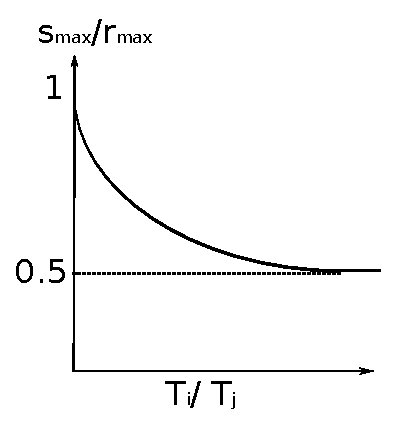
\includegraphics[scale=0.5]{figures/figure14}
\par\end{centering}
\caption{\label{fig14}Effect of $\left\lceil\frac{T_{i}}{T_{j}}\right\rceil$ on
$\frac{s_{max}}{r_{max}}$}
\end{figure}


\subsection{RCM versus Lock-Free}
\label{rcm_vs_lock_free}
\begin{clm}
For RCM's schedulability to be better or equal to that of~\cite{key-5}'s retry-loop lock-free approach, the size of $s_{max}$ must not exceed one half of that of $r_{max}$ for all cases.
However, the size of $s_{max}$ can be larger than that of $r_{max}$, depending on the number of accesses to a task $T_i$'s shared objects from other tasks.
\end{clm}
\begin{proof}
Equation (\ref{eq20}) is upper bounded by:
 \begin{equation}
\sum_{\left(\tau_{j}\in\gamma_{i}\right)\wedge\left(p_{j}> p_{i}\right)}\left(\left\lceil\frac{T_{i}-c_{j}}{T_{j}}\right\rceil+1\right).2.\beta_{i,j}.s_{max}
\label{eq34}\end{equation}

Consider the same assumptions as in Section~\ref{sub:G-EDF-scheduler-with}.
Let $\alpha_{rma}=\sum_{\left(\tau_{j}\in\gamma_{i}\right)\wedge\left(p_{j}> p_{i}\right)}\left(\left\lceil\frac{T_{i}-c_{j}}{T_{j}}\right\rceil+1\right).2.\beta_{i,j}$. Now, the ratio $s_{max}/r_{max}$ is upper bounded by:
\begin{equation}
\frac{s_{max}}{r_{max}}\le\frac{\sum_{T_{i}}\alpha_{free}/t\left(T_{i}\right)}{\sum_{T_{i}}\alpha_{rma}/t\left(T_{i}\right)}
\label{eq35}\end{equation}

The main difference between RCM and lock-free is that RCM is affected only by the higher priority tasks, while lock-free is affected by all tasks (just as in ECM). 
Besides, the RCM
is still affected by $2.\beta_{i,j}$ (just as in ECM).
The subtraction of $c_{j}$ in the numerator in (\ref{eq34}) may not
have a significant effect on the ratio of (\ref{eq35}), as the loop retry 
cost can also be modified to account for the effect of the first interfering
instance of task $T_{j}$. 
%%BR: In this paragraph, why don't you say "RCM" instead of "RMA CM"???


%%BR: Again, in the rest of this section, you can say "RCM" instead of "RMA CM"???
Therefore, 
$\alpha_{free} = \sum_{\tau_{j}\in\gamma_{i}}\left(\left\lceil\frac{T_{i}-c_j}{T_{j}}\right\rceil + 1 \right)\beta_{i,j}$.

Let tasks in the denominator of (\ref{eq35}) be given indexes $k$ instead of $i$, and $l$ instead of $j$. Let tasks in both the numerator and denominator of (\ref{eq35}) be arranged in the non-increasing priority order, so that $i=k$ and $j=l$. Let $\alpha_{free}$, in (\ref{eq35}), be divided into two parts: $\bar{\alpha}_{free}$ that contains only tasks with priority higher than $\tau_i$, and $\hat{\alpha}_{free}$ that contains only tasks with priority lower than $\tau_i$. Now, (\ref{eq35}) becomes:
\begin{eqnarray}
\frac{s_{max}}{r_{max}} & \le & \frac{\sum_{\tau_{i}}(\bar{\alpha}_{free}+\hat{\alpha}_{free})/T_{i}}{\sum_{\tau_{k}}\alpha_{rma}/T_{k}}\nonumber \\
 & = & \frac{1}{2}+\frac{\sum_{\tau_{i}}\hat{\alpha}_{free}/T_{i}}{\sum_{\tau_{k}}\alpha_{rma}/T_{k}}\label{eq36}\end{eqnarray}

For convenience, we introduce the following notations:
\begin{eqnarray}
\zeta_{1}& = & \sum_{\tau_{i}}\frac{\sum_{\left(\tau_{j}\in\gamma_{i}\right)\wedge\left(p_{j}<p_{i}\right)}\left(\left\lceil\frac{T_{i}-c_{j}}{T_{j}}\right\rceil+1\right)\beta_{i,j}}{T_{i}}\nonumber\\
& = & \sum_{T_i} \hat{\alpha}_{free}/T_i
\nonumber\\
\zeta_{2} 
& = & \sum_{\tau_{k}}\frac{\sum_{\left(\tau_{l}\in\gamma_{k}\right)\wedge\left(p_{l}>p_{k}\right)}\left(\left\lceil\frac{T_{k}-c_{l}}{T_{l}}\right\rceil+1\right)\beta_{k,l}}{T_{k}}\nonumber\\
& = & \frac{1}{2}\sum_{\tau_k} \alpha_{rma}/T_k\nonumber
\end{eqnarray}
$\tau_{j}$ is of lower priority than $\tau_{i}$, which means $D_{j}>D_{i}$. Under G-RMA, this means, $T_{j}>T_{i}$.
Thus, $\left\lceil\frac{T_{i}-c_{j}}{T_{j}}\right\rceil=1$ for
all $\tau_{j}$ and $\zeta_{1}=\sum_{\tau_{i}}(\sum_{(\tau_{j}\in\gamma_{i})\wedge(p_{j}<p_{i})}(2.\beta_{i,j}))/T_{i}$.
Since $\zeta_{1}$ contains all $\tau_{j}$ of lower priority than
$\tau_{i}$ and $\zeta_{2}$ contains all $\tau_{l}$ of higher priority than $\tau_{k}$, 
and tasks are arranged in the non-increasing priority order, then for each $\tau_{i,j}$, there exists $\tau_{k,l}$ such
that $i=l$ and $j=k$. Figure~\ref{fig:matrix-example} illustrates this, where 0 means that the pair $i,j$ 
%%BR: Whenever you say "...pair i,j,... say "...pair $(i,j)$...." The brackets help with clarity. Do this fix throughout. 
does not exist in $\zeta_{1}$,
and the pair $k,l$ does not exist in $\zeta_{2}$' (i.e., 
there is no task $\tau_l$ that is going to interfere with $\tau_k$ in $\zeta_2$), 
and 1 means the opposite. 

\begin{figure}[htbp]
\centering
\begin{tabular}{ccc}
$\begin{array}{cccccc}
 & j & 1 & 2 & \cdots & n\\
i\\
1 &  & 0 & 1 & \cdots & 1\\
2 &  & 0 & 0 & \ddots & \vdots\\
\vdots &  & \vdots & \vdots & \ddots & 1\\
n &  & 0 & 0 & \cdots & 0\end{array}$ &  & $\begin{array}{cccccc}
 & l & 1 & 2 & \cdots & n\\
k\\
1 &  & 0 & 0 & \cdots & 0\\
2 &  & 1 & 0 &  & \vdots\\
\vdots &  & \vdots & \ddots & \ddots & 0\\
n &  & 1 & \cdots & 1 & 0\end{array}$\tabularnewline
\end{tabular}
\caption{\label{fig:matrix-example} Task association for lower priority tasks than $T_i$ and higher priority tasks than $T_k$}
\end{figure}

Thus, it can be seen that both the matrices are transposes of
each other. Consequently, for each $\beta_{i,j}$, there exists $\beta_{k,l}$
such that $i=l$ and $j=k$. But the number of times $\tau_{j}$ accesses
a shared object with $\tau_{i}$ may not be the same as the number of times
$\tau_{i}$ accesses that same object. Thus, $\beta_{i,j}$ does not have
to be the same as $\beta_{k,l}$, even if $i,j$ and $k,l$ are transposes 
of each other. Therefore, we can analyze the behavior of $s_{max}/r_{max}$ based on the three parameters $\beta_{i,j}$, $\beta_{k,l}$, and $\left\lceil\frac{T_{k}-c_{l}}{T_{l}}\right\rceil$.
If $\beta_{i,j}$ is increased so that $\beta_{i,j}\rightarrow\infty$,
$\therefore\,(\ref{eq36})\rightarrow\infty$.
This is because, $\beta_{i,j}$ represents the number of times a lower priority task $\tau_{j}$ accesses 
shared objects with the higher priority task $\tau_{i}$. 
While this number has a greater effect in lock-free, it does not have any effect under RCM, because lower priority tasks do not affect higher priority
ones, so $s_{max}$ is allowed to be much greater than $r_{max}$.

Although the minimum value for $\beta_{i,j}$ is 1, mathematically, if $\beta_{i,j}\rightarrow0$, then $(\ref{eq36})\rightarrow1/2$.
Here, changing $\beta_{i,j}$ does not affect the retry cost of RCM, but it does affect the retry cost of lock-free, because the contention between tasks is reduced. Thus, $s_{max}$ is reduced in this case to
a little more than half of $r_{max}$ (``a little more''
because the minimum value of $\beta_{i,j}$ is actually 1, not 0).


The change of $s_{max}/r_{max}$ with respect to $\beta_{i,j}$ is shown in Figure~\ref{fig15-a}.
If $\beta_{k,l}\rightarrow\infty$, then (\ref{eq36})$\rightarrow1/2$.
This is because, $\beta_{k,l}$ represents the number of times
a higher priority task $\tau_{l}$ accesses shared objects with a lower
priority task $\tau_{k}$. Under RCM, this will increase the retry 
cost, thus reducing $s_{max}/r_{max}$. But if $\beta_{k,l}\rightarrow0$, then (\ref{eq36})$\rightarrow\infty$. This is due to the lower contention from a higher priority task $\tau_{l}$ to a lower priority task $\tau_{k}$, which reduces the retry cost under RCM and allows $s_{max}$ to be very large compared with $r_{max}$. Of course, the actual minimum value for $\beta_{k,l}$ is 1, and is illustrated in Figure~\ref{fig15-b}.

The third parameter that affects $s_{max}/r_{max}$ is $T_{k}/T_{l}$.
If $T_{l}\ll T_{k}$, then $\left\lceil\frac{T_{k}-c_{l}}{T_{l}}\right\rceil\rightarrow\infty$,
and $(\ref{eq36})\rightarrow1/2$. This is due to a high number
of interferences from a higher priority task $\tau_{l}$ to a lower priority
one $\tau_{k}$, which increases the retry cost under RMA CM, and consequently reduces $s_{max}/r_{max}$. 

If $T_{l}=T_{k}$ (which is
the maximum value for $T_{l}$ as $D_{l}\le D_{k}$, because
$\tau_{l}$ has a higher priority than $\tau_{k}$), then $\left\lceil\frac{T_{k}-c_{l}}{T_{l}}\right\rceil\rightarrow1$
and $\zeta_2=\sum_{\tau_{k}}\frac{\sum_{\left(\tau_{l}\in\gamma_{k}\right)\wedge\left(p_{l}>p_{k}\right)}2\beta_{k,l}}{t_{k}}$. 
This means that the system will be controlled by only two parameters, $\beta_{i,j}$, and $\beta_{k,l}$, as in the previous two cases, shown in Figures~\ref{fig15-a} and~\ref{fig15-b}. Claim follows.
\end{proof}

\begin{figure}
\begin{centering}
\subfigure[\label{fig15-a}]{\begin{centering}
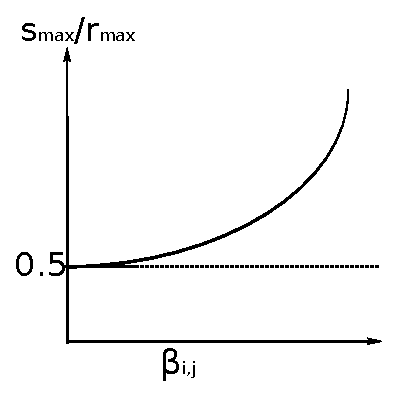
\includegraphics[scale=0.5]{figures/figure15-a}
\par\end{centering}
}\subfigure[\label{fig15-b}]{\begin{centering}
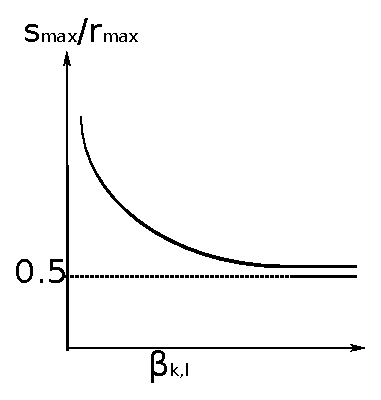
\includegraphics[scale=0.5]{figures/figure15-b}
\par\end{centering}
}
\par\end{centering}
\centering{}\caption{\label{fig15}Change of $s_{max}/r_{max}$: a) $\frac{s_{max}}{r_{max}}$
versus $\beta_{i,j}$ and b) $\frac{s_{max}}{r_{max}}$ versus $\beta_{k,l}$}
%%BR: I updated the caption, correct?
\end{figure}

\subsection{FMLP \& OMLP versus ECM and RCM
}

\begin{clm}
For ECM's schedulability to be better or equal to that of FMLP or OMLP, 
$s_{max}/|s\_\theta|_{max}$ (in case of FMLP), where $|s\_\theta|_{max}$ be the maximum short request by any task, and $s_{max}/L_{max}$ (in case of OMLP) must  not exceed $O(\frac{m}{n})$, where $L_{max}=max_{\forall i,\forall k}L_{i,k}$. For RCM's schedulability  
to be better or equal  
to that of OMLP, $s_{max}/L_{max}$ must not exceed $O(\frac{m}{n})$.
\end{clm}
\begin{proof}
As FMLP is used with G-EDF (GSN-EDF), we compare only ECM 
against it. 
%%BR: "...we compare only ECM against it."??? 
First, we derive upper bounds for the blocking parameters of FMLP. When requests are non-nested, each resource (short or long) will be contained in its own group. Let $N_{i,s}$ be the number of times a task $T_{i}$ requests a short
resource, $|s\_\theta|_{i,max}$ be the maximum request for a
short resource by $T_{i}$, $\alpha_{bw}=N_{i,s}.(m-1)$. Now, FMLP's three  blocking terms, described in Section~\ref{global-fmlp}, are upper bounded as follows:
\begin{eqnarray*}
BW(T_{i}) & \le & \sum_{s\_\theta\in\theta_{i}}(m-1).|s\_\theta|_{i,max}\\
 & = & N_{i,s}.(m-1).|s\_\theta|_{i,max}\\
 & \le & N_{i,s}.(m-1).|s\_\theta|_{max}\\
& = & \alpha_{bw}.|s\_\theta|_{max}
 \end{eqnarray*}
\begin{eqnarray*}
NPB\left(T_{i}\right) & \le & \left(1+N_{i,l}\right).max\left(BW_{k\ne i}\left(T_{k}\right)+|s\_\theta|_{k,max}\right)\\
 & \le & \left(1+N_{i,l}\right).max\left(BW_{k\ne i}\left(T_{k}\right)+|s\_\theta|_{max}\right)\\
 & = & \left(1+N_{i,l}\right).|s\_\theta|_{max}.max_{k\ne i}\left(N_{k,s}.\left(m-1\right)+1\right)\\
 & = & \alpha_{npb}.|s\_\theta|_{max}
 \end{eqnarray*}
 where $\alpha_{npb}=\left(1+N_{i,l}\right).max_{k\ne i}\left(N_{k,s}.\left(m-1\right)+1\right)$.
\begin{eqnarray*}
DB\left(T_{i}\right) & \le & N_{i,l}.\left(n-1\right).|l\_\theta|_{i,max}\\
 & \le & N_{i,l}.\left(n-1\right).|l\_\theta|_{max}\\
 \end{eqnarray*}
If $|l\_\theta|_{max}\le c1.|s\_\theta|_{max}$, where $c1$ is the
minimum constant that satisfies this relation, then
\begin{eqnarray*}
DB\left(T_{i}\right)& \le & N_{i,l}.\left(n-1\right).c1.|s\_\theta|_{max}\\
& = & \alpha_{db}.|s\_\theta|_{max}
\end{eqnarray*}
where $\alpha_{db}=N_{i,l}.\left(n-1\right).c1$. 

The total blocking time of each task is added to the task execution time, and
as before, we compare the total utilization of the G-EDF system (with both contention managers) against that under FMLP. 

Now, for ECM's schedulability to be better than FMLP,
\begin{equation}
 \frac{s_{max}}{|s\_\theta|_{max}}\le
 \frac{\sum_{T_{i}}\left(\alpha_{bw}+\alpha_{npb}+\alpha_{db}\right) \Big/t(T_{i})}{\sum_{T_{i}}\alpha_{edf} \Big/t(T_{i})}
 \label{eq38} \end{equation}

From (\ref{eq38}), it can be seen that $T_{i}$'s blocking time,
under FMLP, depends on $m,\, n$ and the number of times it requests resources
(in contrast to ECM, 
%%BR: "...contrast to ECM,..."???  
under which, $T_i$'s retry cost depends on the number of times a conflicting task $T_{j}$ requests resources). Thus, if $N_{i,s},\, N_{i,l}$, 
and $N_{k,s}$ can all be upper bounded by some constant $C_{2}$,
which is the maximum number of times any task $T_{i}$ can request a short
or long resource, then the numerator in (\ref{eq38}) 
is $O(n(n+m))$, while the denominator is $O(n^{2})$. Therefore:
\begin{equation}
\frac{s_{max}}{|s\_\theta|_{max}}=O\left(\frac{m}{n} \right)
\label{eq45}
\end{equation}
This means that, for $n<m$, the contention between tasks under both STM and
FMLP is low (even for short resources under FMLP), but FMLP is more affected
by $NTB$. When $n>m$, contention increases, but FMLP arranges
requests in a FIFO queue, so it is less affected than ECM, 
%%BR: "..than ECM,...???
which
suffers from conflicting tasks and instances
of each conflicting one. FMLP is not affected by the number of instances
of each conflicting task.

%%%%
Since OMLP's blocking time is bounded by (\ref{eq29}) \[ \therefore 
%\;
bi\le2.\left(m-1\right).L_{max}\sum_{k=1}^{q}N_{i,k}\]
%%BR: THis sentence is awkward. Why don't you say "Let  \[L_{max}=..... Since OMLP's blocking time is ..., \therefore.."


For ECM's schedulability to be better than global OMLP:
\begin{equation}
\frac{s_{max}}{L_{max}}\le\frac{\sum_{T_{i}}\left(2.\left(m-1\right)\sum_{k=1}^{q}N_{i,k}\right) \Big/t\left(T_{i}\right)}{\sum_{T_{i}}\alpha_{edf} \Big/t\left(T_{i}\right)}\label{eq40}\end{equation}

For RCM, the ratio is:
\begin{equation}
\frac{s_{max}}{L_{max}}\le\frac{\sum_{T_{i}}\left(2.\left(m-1\right)\sum_{k=1}^{q}N_{i,k}\right) \Big/t\left(T_{i}\right)}{\sum_{T_{i}}\alpha_{rma} \big/t\left(T_{i}\right)}\label{eq41}\end{equation}


If $\sum_{k=1}^{q}N_{i,k}$ is upper bounded by $C_{3}$, which is
a constant representing the maximum total number of requests for resources
by any task $T_{i}$, then:
\begin{equation}
\frac{s_{max}}{L_{max}}=O\left(\frac{nm}{n^{2}}\right)=O\left(\frac{m}{n}\right)
\label{eq46}
\end{equation}
for each of (\ref{eq40}) and (\ref{eq41}). Claim follows.
\end{proof}


\subsection{G-EDF/LCM versus lock-free synchronization}

We consider the lock-free retry-loop approach for G-EDF in~\cite{key-5}, where a retry upper bound is developed by computing the worst-case number of tasks that can execute within one period of the task being considered. This lock-free approach is the most relevant to our work.

\begin{clm}
If $r_{max}$ is the maximum execution cost of a single iteration of any retry loop of any task in the retry-loop lock-free algorithm in~\cite{key-5}, then G-EDF/LCM can provide equal or higher $\frac{s_{max}}{r_{max}}$ than what is provided by ECM
%~\cite{stmconcurrencycontrol:emsoft11}. In some cases, G-EDF/LCM can even provide higher $s_{max}$ than $r_{max}$.
\end{clm}
%
\begin{proof}
From~\cite{key-5}, the retry-loop lock-free algorithm is upper bounded by:
\begin{equation}
RL(T_i)=\sum_{\tau_{h}\in\gamma_{i}}\left(\left\lceil\frac{T_{i}}{T_{h}}\right\rceil +1\right)\beta_{i,h}r_{max}
\label{eq32}\end{equation}
The final cost of $\tau_i$ due to $\tau_h$ in G-EDF/LCM is upper bounded by (\ref{newcost}). By comparing G-EDF/LCM's total utilization with that of the retry-loop lock-free algorithm, we get:
\begin{equation*}
%& 
 \forall \tau_{i}\frac{\sum_{\forall \tau_{h}\in\gamma_{i}}\left((1-\alpha_{min})+\left\lceil\frac{T_{i}}{T_{h}}\right\rceil(1+\alpha_{max})\right)\beta_{i,h}s_{max}}{T_{i}}
%& 
\le  \forall \tau_{i}\frac{\sum_{\forall \tau_{h}\in\gamma_{i}}\left(\left\lceil\frac{T_{i}}{T_{h}}\right\rceil+1\right)\beta_{i,h}r_{max}}{T_{i}}\end{equation*}
%
\begin{eqnarray*}
\therefore\frac{s_{max}}{r_{max}}\le\frac{\forall \tau_{i}\frac{\sum_{\forall \tau_{h}\in\gamma_{i}}\left(\left\lceil\frac{T_{i}}{T_{h}}\right\rceil+1\right)\beta_{i,h}}{T_{i}}}{\forall \tau_{i}\frac{\sum_{\forall \tau_{h}\in\gamma_{i}}\left((1-\alpha_{min})+\left\lceil\frac{T_{i}}{T_{h}}\right\rceil(1+\alpha_{max})\right)\beta_{i,h}}{T_{i}}}
\end{eqnarray*}
Using (\ref{edf-lcm-ecm}), we choose $1-\alpha_{min}=\left\lceil\frac{T_{i}}{T_{h}}\right\rceil(1-\alpha_{max})-\Delta\left\lceil\frac{T_{i}}{T_{h}}\right\rceil$, where $\Delta>0$. Then:
\begin{eqnarray*}
\frac{s_{max}}{r_{max}} & \le & \frac{\forall \tau_{i}\frac{\sum_{\forall \tau_{h}\in\gamma_{i}}\left(\left\lceil\frac{T_{i}}{T_{h}}\right\rceil+1\right)\beta_{i,h}}{T_{i}}}{(2-\Delta)\forall \tau_{i}\frac{\sum_{\forall \tau_{h}\in\gamma_{i}}\left\lceil\frac{T_{i}}{T_{h}}\right\rceil\beta_{i,h}}{T_{i}}}\nonumber\\
 & = & \frac{\forall \tau_{i}\frac{\sum_{\forall \tau_{h}\in\gamma_{i}}\left\lceil\frac{T_{i}}{T_{h}}\right\rceil\beta_{i,h}}{T_{i}}}{(2-\Delta)\forall \tau_{i}\frac{\sum_{\forall \tau_{h}\in\gamma_{i}}\left\lceil\frac{T_{i}}{T_{h}}\right\rceil\beta_{i,h}}{T_{i}}}
 +  \frac{\forall \tau_{i}\frac{\sum_{\forall \tau_{h}\in\gamma_{i}}\beta_{i,h}}{T_{i}}}{(2-\Delta)\forall \tau_{i}\frac{\sum_{\forall \tau_{h}\in\gamma_{i}}\left\lceil\frac{T_{i}}{T_{h}}\right\rceil\beta_{i,h}}{T_{i}}}\nonumber\\
 & = & \frac{1}{2-\Delta}+\frac{\forall \tau_{i}\frac{\sum_{\forall \tau_{h}\in\gamma_{i}}\beta_{i,h}}{T_{i}}}{(2-\Delta)\forall \tau_{i}\frac{\sum_{\forall \tau_{h}\in\gamma_{i}}\left\lceil\frac{T_{i}}{T_{h}}\right\rceil\beta_{i,h}}{T_{i}}}
 \label{g-edf/lcm-retry}\end{eqnarray*}

If $\left\lceil\frac{T_i}{T_h}\right\rceil\rightarrow1$ (as there must be at least one instance of $\tau_h$ conflicting with $\tau_i$), then: 
\begin{equation*}
\frac{s_{max}}{r_{max}}\rightarrow \frac{2}{2-\Delta}
\end{equation*}
Thus, $0 \le \Delta <2$. If $\Delta\rightarrow0$, $\therefore \frac{s_{max}}{r_{max}}\rightarrow1$. But if $\Delta\rightarrow2$, $\therefore \frac{s_{max}}{r_{max}}\rightarrow\infty$. This means that, in case of low conflict among tasks and by proper choice of $\Delta$, the length of $s_{max}$ can be equal to or much greater than the length of $r_{max}$.

If $\left\lceil\frac{T_i}{T_h}\right\rceil\rightarrow\infty$, then:
\begin{equation*}
\frac{s_{max}}{r_{max}}\rightarrow \frac{1}{2-\Delta}
\end{equation*}
Thus, $\Delta$ is still in $[0,2[$, and if $\Delta\rightarrow0$, $\therefore \frac{s_{max}}{r_{max}}\rightarrow0.5$. But if $\Delta\rightarrow2$, $\therefore \frac{s_{max}}{r_{max}}\rightarrow\infty$. So, in case of high conflict among tasks, the minimum upper bound for the length of $s_{max}$ is half the length of $r_{max}$. By proper choice of $\Delta$, the length of $s_{max}$ can be much greater than that of $r_{max}$.

Thus, we see that, in G-EDF/LCM and by the proper choice of $\Delta$ (consequently, by the proper choice of $\alpha_{min}$ and $\alpha_{max}$), the length of $s_{max}$ ranges from half the length of $r_{max}$ to much higher multiples of $r_{max}$. On the other hand, in ECM
%~\cite{stmconcurrencycontrol:emsoft11}
, the length of $s_{max}$ ranges only from half the length of $r_{max}$ to the full length of $r_{max}$. Claim follows.
\end{proof}

\subsection{G-RMA/LCM versus lock-free synchronization}
\begin{clm}
While the minimum upper bound on $s_{max}/r_{max}$ in RCM is 0.5
%~\cite{stmconcurrencycontrol:emsoft11}
, G-RMA/LCM achieves a higher minimum upper bound of $1/(1+\alpha_{max})$ on $s_{max}/r_{max}$ by proper choice of $\alpha_{max}$. This helps to achieve a better or equal schedulability than the retry-loop lock-free algorithm. Similarly to RCM, G-RMA/LCM can increase the length of $s_{max}$ over $r_{max}$ in some cases, 
which happens when abortion of lower priority tasks effect is reduced and $\alpha_{min}$ is increased.
\end{clm}
%
\begin{proof}
$RC(T_{i})$ for G-RMA/LCM is upper bounded by (\ref{eq68}),
and $RL(T_{i})$ for retry-loop lock-free algorithm is upper bounded
by (\ref{eq32}), which is re-written here as:
\begin{equation}
RL(T_{i})=\sum_{\tau_{v}\in\gamma_{i}}\left(\left\lceil\frac{T_{i}}{T_{v}}\right\rceil+1\right)\beta_{iv}r_{max}\label{eq72}
\end{equation}
The set of tasks $\tau_{v}\in\gamma_{i}$ are composed of tasks with  higher priority than $\tau_{i}$, and are denoted as $\tau_{j}$, to be consistent with G-RMA/LCM's index notation, and tasks with lower priority than $\tau_{i}$, which are denoted as $\tau_{h}$. Thus, (\ref{eq72}) can be re-written as:
\begin{equation}
RL(T_{i})  =  \sum_{\forall \tau_{j}^{*}}\left(\left\lceil\frac{T_{i}}{T_{j}}\right\rceil+1\right)\beta_{ij}r_{max}
 +  \sum_{\forall\bar{\tau}_{h}}\left(\left\lceil\frac{T_{i}}{T_{h}}\right\rceil+1\right)\beta_{ih}r_{max}\label{eq73}\end{equation}


Assume that $\lambda_{3}(i,j)=\left(\left\lceil\frac{T_{i}}{T_{j}}\right\rceil+1\right)\beta_{ij}$
and $\chi_{3}(i,h)=\left(\left\lceil\frac{T_{i}}{T_{h}}\right\rceil+1\right)\beta_{ih}$.
To determine when the schedulability of G-RMA/LCM will
be better or equal to that of retry-loop lock-free, we compare the total
utilization of both:
\begin{eqnarray*}
& & \sum_{\forall \tau_{i}}\frac{\sum_{\forall \tau_{j}^{*}}\Big(\lambda_{3}(i,j)(1+\alpha_{max})len(s_{max})\Big)}{T_{i}}+ \sum_{\forall \tau_{i}}\frac{\sum_{\forall\bar{\tau}_{h}}\Big(\chi_{3}(i,h)(1-\alpha_{min})len(s_{max})\Big)}{T_{i}}\\
& \le & r_{max}\sum_{\forall \tau_{i}}\frac{\sum_{\tau_{j}^{*}}\lambda_{3}(i,j)+\sum_{\bar{\tau}_{h}}\chi_{3}(i,h)}{T_{i}}\end{eqnarray*}


\begin{equation*}
\therefore\frac{s_{max}}{r_{max}} \le  
\frac{\sum_{\forall \tau_{i}}\frac{\sum_{\tau_{j}^{*}}\lambda_{3}(i,j)+\sum_{\bar{\tau}_{h}}\chi_{3}(i,h)}{T_{i}}}{\sum_{\forall \tau_{i}}\frac{\sum_{\forall \tau_{j}^{*}}(\lambda_{3}(i,j)(1+\alpha_{max}))+\sum_{\forall\bar{\tau}_{h}}(\chi_{3}(i,h)(1-\alpha_{min}))}{T_{i}}} \end{equation*}


Since task relative deadline equals task period, and $\tau_{h}$ is of lower priority than $\tau_{i}$, $T_{i}\le T_{h}$. Therefore, $\left\lceil\frac{T_{i}}{T_{h}}\right\rceil=1$ for any $\tau_{i}$ and $\tau_{h}$. Thus:
\begin{equation}
\frac{s_{max}}{r_{max}}\le\frac{\sum_{\forall \tau_{i}}\frac{\sum_{\forall \tau_{j}^{*}}\lambda_{3}(i,j)+2\sum_{\forall\bar{\tau}_{h}}\beta_{ih}}{T_{i}}}{\sum_{\forall \tau_{i}}\frac{\sum_{\forall \tau_{j}^{*}}(\lambda_{3}(i,j)(1+\alpha_{max}))+2\sum_{\forall\bar{\tau}_{h}}((1-\alpha_{min})\beta_{ih})}{T_{i}}}\label{eq74}\end{equation}


If the following inequality holds:
\begin{equation}
\frac{s_{max}}{r_{max}}\le\frac{\sum_{\forall \tau_{i}}\frac{\sum_{\forall \tau_{j}^{*}}\lambda_{3}(i,j)+2\sum_{\forall\bar{\tau}_{h}}\beta_{ih}}{T_{i}}}{\sum_{\forall \tau_{i}}\frac{\sum_{\forall \tau_{j}^{*}}(\lambda_{3}(i,j)(1+\alpha_{max}))+2\sum_{\forall\bar{\tau}_{h}}((1+\alpha_{max})\beta_{ih})}{T_{i}}}\label{eq74-1}\end{equation}
where $1-\alpha_{min}$ in the denominator of the right hand
side of (\ref{eq74}) is replaced by $1+\alpha_{max}$,
then (\ref{eq74}) holds, because the right hand side
of (\ref{eq74-1}) is lower or equal to the right hand
side of (\ref{eq74}). Thus, 
\begin{eqnarray}
\frac{s_{max}}{r_{max}} & \le & \frac{\sum_{\forall \tau_{i}}\frac{\sum_{\forall \tau_{j}^{*}}\lambda_{3}(i,j)+2\sum_{\forall\bar{\tau}_{h}}\beta_{ih}}{T_{i}}}{(1+\alpha_{max})\sum_{\forall \tau_{i}}\frac{\sum_{\forall \tau_{j}^{*}}\lambda_{3}(i,j)+2\sum_{\forall\bar{\tau}_{h}}\beta_{ih}}{T_{i}}}\label{eq76}\end{eqnarray}
\begin{eqnarray}\therefore\frac{s_{max}}{r_{max}} & \le & \frac{1}{1+\alpha_{max}}\label{eq75}\end{eqnarray}

Since $0\le\alpha_{max}\le1$, and by proper choice of $\alpha_{max}$, the minimum upper bound on $\frac{s_{max}}{r_{max}}$ is higher
than 0.5. Thus, the length of $s_{max}$ can be kept higher than half the length of $r_{max}$, which is higher than that achieved in the specific cases of RCM. 
%~\cite{stmconcurrencycontrol:emsoft11}.
(In fact, $\frac{s_{max}}{r_{max}}$ is higher than $\frac{1}{1+\alpha_{max}}$, because the right hand side of (\ref{eq74}) is the actual
upper limit to $\frac{s_{max}}{r_{max}}$, not the right hand side
of (\ref{eq76})).
(\ref{eq75}) represents the general case for comparison between G-RMA/LCM and retry-loop lock-free. (\ref{eq75}) yields the
higher upper limit on $\frac{s_{max}}{r_{max}}$ as 1, which means
that the maximum allowed length for $s_{max}$, for G-RMA/LCM's schedulability to be better or equal to that of RCM, is the length of $r_{max}$. However, considering the special cases in Section~\ref{rcm_vs_lock_free},
%~\cite{stmconcurrencycontrol:emsoft11},
 this can be changed as follows.

From (\ref{eq74}), it appears that $\frac{s_{max}}{r_{max}}$ depends on $\beta_{ij}$, $\beta_{ih}$,
$\left\lceil\frac{T_{i}}{T_{j}}\right\rceil$, $\alpha_{max}$, and $\alpha_{min}$. The
minimum value for $\beta_{ij}$ and $\beta_{ih}$ is 1, as there must
be at least one shared resource between $\tau_{i},\tau_{j}$ and $\tau_{i},\tau_{h}$. 
$\beta_{ij}\rightarrow0$, which means that the value of $\beta_{ij}$ is very small compared to that of $\beta_{ih}$, and $\beta_{ih}\rightarrow0$, which means that the value of $\beta_{ih}$ is very small compared to that of $\beta_{ij}$. Also, if $\beta_{ij}\rightarrow\infty$ ($\beta_{ih}\rightarrow\infty$),
then the value of $\beta_{ij}$ ($\beta_{ih}$) is very large compared
to that of $\beta_{ih}$ ($\beta_{ij}$). If $\beta_{ij}\rightarrow\infty$
or $\beta_{ih}\rightarrow0$ (which can happen if higher priority
tasks tend to access shared resources more frequently than lower
priority tasks), then (\ref{eq74}) $\rightarrow$ $\frac{s_{max}}{r_{max}}\le\frac{1}{1+\alpha_{max}}$, which is the same as the general boundary from (\ref{eq75}).

If $\beta_{ij}\rightarrow0$ or $\beta_{ih}\rightarrow\infty$,
which happens if higher priority tasks tend to access shared resources rarely compared with lower priority tasks, then (\ref{eq74})
$\rightarrow\frac{s_{max}}{r_{max}}\le\frac{1}{1-\alpha_{min}}$. If $\alpha_{min}\rightarrow0$,
then the length of $s_{max}$ can be at most as that of $r_{max}$. 

The physical interpretation of these parameters (i.e., $\beta_{ij}\rightarrow0$
or $\beta_{ih}\rightarrow\infty$ and $\alpha_{min}\rightarrow0$)
is that the effect of blocking in G-RMA/LCM is very large compared
to that of interference, and it is even increased by making $\alpha_{min}\rightarrow0$. This means that an atomic section $s_{j}^{l}(\theta)$, belonging
to a higher priority task $T_{j}$, would suffer the maximum blocking
time from any 
atomic section $s_{i}^{k}(\theta)$ belonging to a lower
priority task $T_{i}$, because $s_{j}^{l}(\theta)$ will have to
wait for almost the whole length of $s_{i}^{k}(\theta)$ in the worst
case of blocking.

Since the retry-loop lock-free method also suffers blocking from 
lower priority tasks whose effect is approximately the same as lower priority tasks in G-RMA/LCM (as $\alpha_{min}\rightarrow0$), this will cause the lengths of $s_{max}$ and $r_{max}$ to be approximately the same. If $\alpha_{min}\rightarrow1$,
then $\frac{s_{max}}{r_{max}}\le\infty$, which means that the length of
$s_{max}$ can be much greater than that of $r_{max}$. 

The physical interpretation for these parameters (i.e., $\beta_{ij}\rightarrow0$
or $\beta_{ih}\rightarrow\infty$ and $\alpha_{min}\rightarrow1$)
is that the effect of blocking in G-RMA/LCM is very large compared
to the effect of interference. If $\alpha_{min}\rightarrow1$, then
an atomic section $s_{j}^{l}(\theta)$ will be blocked by another
one $s_{i}^{k}(\theta)$ for a very short time length (almost 0). This will significantly reduce the effect of lower priority tasks,
in contrast to the retry-loop lock-free algorithm, where lower priority
tasks still affect the retry cost. Thus, the length of $s_{max}$ can be much greater than that of $r_{max}$
to achieve higher schedulability than the lock-free method.


If $\left\lceil\frac{T_i}{T_j}\right\rceil\rightarrow1$, then (\ref{eq74})  becomes:
\begin{equation*}
\frac{s_{max}}{r_{max}}\le\frac{\sum_{\forall \tau_{i}}\frac{\sum_{\tau_{j}^*}\beta_{ij}+\sum_{\bar{\tau}_{h}}\beta_{ih}}{T_{i}}}{\sum_{\forall \tau_{i}}\frac{(1+\alpha_{max})\sum_{\tau_{j}^*}\beta_{ij}+(1-\alpha_{min})\sum_{\bar{\tau}_{h}}\beta_{ih}}{T_{i}}}
\end{equation*}
This means that, the relative schedulability of G-RMA/LCM and the retry-loop lock-free method depends on $\beta_{ij}$, $\beta_{ih}$, $\alpha_{max}$, and $\alpha_{min}$, as explained above. 
If $\left\lceil\frac{T_i}{T_j}\right\rceil\rightarrow\infty$,
then (\ref{eq74})$\rightarrow\frac{s_{max}}{r_{max}}\le\frac{1}{1+\alpha_{max}}$, which is the same as the general boundary derived in (\ref{eq75}).

The claim follows from the analysis for the general and special cases.
\end{proof}
\end{comment}



\section{Conclusions}
\label{sec:conclusions}

In ECM and RCM, a task incurs at most $2s_{max}$ retry cost for each one of its atomic sections due to conflict
with another task's atomic section. With LCM, this retry cost is reduced to $(1+\alpha_{max})s_{max}$ for each aborted atomic section. In ECM and RCM, tasks do not retry due to lower priority tasks, while in LCM, this happens. In G-EDF/LCM, retrial due to lower priority job is encountered only from a task
$\tau_{j}$'s last instance during $\tau_{i}$'s period. This is not the case with G-RMA/LCM, because,  each higher priority task can be aborted and retried by all lower priority tasks.

Schedulability of G-EDF/LCM and G-RMA/LCM can be better or equal to ECM and RCM, respectively, by proper choices for $\alpha_{min}$ and $\alpha_{max}$. 
%with proper choices for $\alpha_{max}$ and $\alpha_{min}$, 
\begin{comment}
When LCM was compared with lock-free, the minimum upper bound on the length of $s_{max}$ could be more than half the length of $r_{max}$,
which is higher than that achieved in ECM and RCM, and it can even be much larger than $r_{max}$ in both G-EDF/LCM and G-RMA/LCM. While achieving these high values for $s_{max}$ compared to $r_{max}$ is possible in RCM, it is not possible in ECM, as the maximum value for $s_{max}$'s length is $r_{max}$.
\end{comment}

Our work has only further scratched the surface of real-time STM. Our work is analytical, because our question is analytical---i.e., how to increase STM's schedulability advantage through a novel CM design? That said, significant insights can be gained by experimental work, which is outside this work's  scope. For e.g., what are the typical range of values for the different parameters that affect the retry and blocking costs (and hence response time)? How tight is our derived upper bounds in practice? 
What is the most practically suitable
value for $\psi$, $\alpha_{min}$, and $\alpha_{max}$? Is it more suitable to have different $\alpha$s (hence different $\psi$s) for different atomic section lengths, instead of using the normalized atomic section length? 


%\bibliographystyle{acmsmall}
%\bibliography{global_bibliography}

\bibliographystyle{IEEEtran}
\bibliography{IEEEabrv,global_bibliography}

\end{document}
